\section{Authority-Bearing Incident Coordination under Intermittent Connectivity}
\label{sec:problem-analysis}

Rescue-service incident response exposes a design tension between availability and authority. Responders must continue operating under intermittent connectivity, yet authority-bearing incident decisions must remain attributable to a single operational commander.

The target setting is municipal rescue-service incident response, where a regional core supports dispatch and reference data, vehicle edge nodes operate near the incident site, and field tablets attach to local vehicles acting as leaf
clients. Connectivity is intermittent, vehicles may move between wide-area
connectivity, mesh-only contact, and total
isolation~\cite{zimbelman2022mesh,wang2023overview} (Figure~\ref{fig:op-setting}). One vehicle edge node holds
the command role for the incident; we refer to it as the \emph{command edge}. The role can move to another vehicle, but only through an explicit human decision, and the protocol must respect that
operational authority. 

\begin{figure}[ht]
\centering
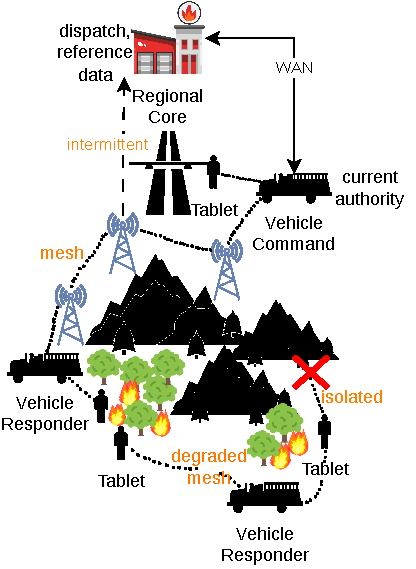
\includegraphics[width=0.72\columnwidth]{figures/operationalSetting.drawio.pdf}
\caption{Operational setting. A regional core supports dispatch and reference data; vehicle edge nodes run near the incident site; tablets attach to a local vehicle. One vehicle holds command authority at any instant. Vehicles simultaneously occupy different connectivity regimes: wide-area backhaul, intermittent backhaul with mesh transit, or total isolation.}
\label{fig:op-setting}
\end{figure}

\subsection{Operational Requirements}
\label{sec:requirements}

Public rescue-service guidance and studies of Swedish rescue-service information
systems motivate the requirements used here~\cite{rsg-rad201,rsg-kommunalplan,pilemalm2014enabling,westman2021mobilisation}.
R1 and R2 follow from mobile-IT and incident-reporting findings that responders need locally available information and durable later documentation~\cite{pilemalm2014enabling,westman2021mobilisation}. R3 follows from decision-provenance requirements and rescue-service command guidance~\cite{naja2010provenance,rsg-rad201,rsg-kommunalplan}.

The externally motivated operational requirements are:
\begin{itemize}
  \item \textbf{\textit{R1 (Offline operation)}} Each tier must keep working from
  previously synchronized data without continuous connectivity.
  \item \textbf{\textit{R2 (Durable forward-only submission)}} Field submissions entered
  on tablets must survive vehicle restart and prolonged partition.
  \item \textbf{\textit{R3 (Attributable command authority)}} Resource assignments,
  status transitions, and hazard annotations must be attributable to one
  operational command authority at any instant.
\end{itemize}

These requirements sit at different layers, by design. R1 and R2 are
availability and durability properties that \systemname{} satisfies with weaker
local and eventual contracts, outside the authority boundary; R3 is a
single-authority property satisfied inside it. The contribution is the M1
state-class partition that lets the three be met by different contracts, rather
than forcing one contract on all incident data.

R3 is not a claim that crisis governance is simple. Incident-command studies and
emergency-management reviews describe hierarchies embedded in multi-actor
response networks, where authority may be shared, delegated, contested, or
legally bounded~\cite{moynihan2008combining,wennman2022organizational,dalessio2024leading}.
Yet emergency-response decision provenance still requires a defined subset of
command decisions to remain attributable to the authority that made
them~\cite{naja2010provenance}; R3 abstracts that accountability property,
authority-bearing writes have one current command authority, while other
coordination need not be single-leader. For \systemname{}, this yields conservative
transfer semantics, a new command edge is accepted only after
operator-initiated promotion, not inferred from reachability.

\subsection{Positioning Relative to Consensus, CRDTs, Local-first, and Emergency Networking}
\label{sec:positioning}

\systemname{} recombines known mechanisms--single-leader replication,
transactional outbox~\cite{richardson2018microservices}, idempotency keys, and
manual fencing--under a domain rule: the command edge is the incident-journal
linearization point. The incident-state entity owns its decision history;
external actors submit forward-only events rather than mutate it
directly~\cite{helland2017life}. The contribution is the M1 state-class
partition and grounding the boundary in external command authority; the
mechanisms themselves are not claimed as novel.

\textit{Consensus and replicated state machines.} Consensus, shared-log, and
chain-replication systems provide replicated agreement and totally ordered logs
under their stated failure
models~\cite{lamport1998parttime,ongaro2014raft,balakrishnan2013tango,vanrenesse2004chain}.
These systems supply stronger ordering than R3 requires, at a cost the workload
does not justify: rescue-service traffic is dominated by reference-data lookups
and append-only reporting, for which quorum agreement and leader election are
over-engineered. Election-based liveness selects a writer by reachability, whereas
R3 fixes the writer by operational command; \S~\ref{sec:eval-raft} measures this
mismatch on a three-voter Raft baseline.

\textit{CRDTs and strong eventual consistency.} CRDT and strong-eventual-consistency work provides convergence for mergeable
replicated state~\cite{almeida2014delta,hanssen2025emergency,almeida2024crdtsurvey}.
It serves R1/R2 well but cannot satisfy R3~\cite{mao2024reliablecrdt}.
Authority-bearing incident decisions such as resource assignments, status
transitions and hazard annotations are non-commutative: there is no
application-defensible merge for two responders setting the same status to
conflicting values. R3 therefore requires attribution and a single authoritative
order, not automatic conflict rejection. AAL's measured path preserves both
conflicting writes in an attributed total order; semantic guards are a disclosed
extension (\S~\ref{sec:non-claims}). Any deterministic merge rule implicitly
invents the authority R3 requires be explicit.

\textit{Offline-first and local-first systems.} Offline-first and local-first
systems prioritize local availability and continued operation under poor
connectivity~\cite{kleppmann2019localfirst,richardson2018microservices}.
They satisfy R1 and R2 and are the right model for reference data, field
submissions, and materialized views. But their design goal is replica
\emph{autonomy}---every node is equally entitled to write and reconcile---which
is precisely the property the command hierarchy rejects for authority-bearing
decisions (R3).

\textit{Why not a centralized backend?} A regional backend cannot hold the
linearization point when it is partitioned from the incident, which is the
common case: vehicles operate hours from dispatch (\S~\ref{sec:introduction}),
and no server can serialize writes it cannot reach. Authority-bearing command
decisions must therefore serialize at the incident during total backhaul
isolation. A backend-authoritative offline-first design has two bad
options. It can block command decisions while isolated, violating R1 for the
command stream. Or it can let field nodes write provisionally and reconcile later,
reintroducing the multi-writer merge problem R3 forbids. \systemname{} places the linearization point at the
command edge precisely so the authoritative order survives backhaul partition;
the regional core still owns reference data, which tolerates the weaker R1 and
R2 contracts.

\textit{Emergency and edge networking.} Closest in setting is emergency and edge
networking. CoNICE~\cite{jahanian2022conice} reaches consensus among
infrastructure-less peers using One-Third-Rule agreement, layered over epidemic
replication, causality metadata, and decision invalidation for long-term
fragmentation. That is substantial machinery when the operational problem already
designates a commander: rescue-service incident command has a designated commander
at every moment, and the network is not permitted to vote on incident decisions,
so CoNICE's no-privileged-peer assumption is exactly the one R3 removes. Public-safety networking and edge/fog
research place resilient
transport and storage near
responders~\cite{kumbhar2015legacy,wang2023overview,sagor2024distressnetng},
addressing R1 transport but not which actor may issue an authority-bearing
decision.

Across these families, each helps responders keep working or order writes, but
none decides \emph{which actor} may issue an authority-bearing decision during a
partition. Primary/backup systems already use manual failover and fencing
tokens~\cite{kleppmann2017ddia}; the distinction here is using operational
command authority to set the linearization boundary while assigning weaker
contracts to non-authority incident data.

\subsection{Assumptions and Design Choices}
\label{sec:assumptions}

These choices are responses to the requirements, not the requirements
themselves. R3 does not require a single-writer database for all incident state;
it requires authority-bearing decisions to remain attributable to the current
command authority. \systemname{} conservatively places the incident-journal
linearization boundary at the command edge, while reference data, field
submissions, and materialized views keep weaker local or eventual contracts. 
% M1 is the state-class partition that chooses which data crosses that boundary;
% M2--M4 implement sequencing, submission, and transfer. The design assumes one
% current command authority, fixed at dispatch and changed only by explicit
% operator decision.

The deployment constraints identified in the introduction are separate. The mesh
should act as routed transit rather than a stretched user network, and the system
must reuse the rescue-service identity infrastructure. Their architectural
consequences---edge cache and local services, tablet/edge outbox and retry, a
single incident-journal writer, mesh-as-transit routing, and mTLS/CA identity
integration---are developed in \S~\ref{sec:architecture}.
